% !TeX root = ../../../main.tex
\section{零过程噪声 Logistic 模型：粒子贫化与稳健性}\label{cw:sec:sim-logistic}
考虑确定性混沌状态演化与非线性观测：
\begin{equation}\label{cw:eq:sim-logistic-model}
\begin{aligned}
&X_k=4X_{k-1}(1-X_{k-1}),\quad X_k\in[0,1],\\
&Y_k=h(X_k)+N_{y,k},\quad h(x)=x^2,\quad
X_0\sim U[0,1],\quad N_{y,k}\sim\mathcal N(0,0.1).
\end{aligned}
\end{equation}
每步均有观测，取 $N=128$，共 $64$ 条独立观测路径，每条 $1000$ 步，每条路径独立运行算法 $32$ 次。观测噪声方差为 $0.1$；BPF 采用每步多项重采样，ETPF 采用一维无正则最优输运。不同粒子位置数按双精度数值精确去重统计。

图~\ref{cw:fig:sim-logistic-robustness} 比较两种算法的误差与粒子多样性，四项误差统计见表~\ref{cw:tab:sim-logistic-errors}。

\begin{table}[!htb]
\centering\wuhao
\caption{Logistic 模型的四项误差与实测总 MSE，第 $1$--$1000$ 步平均。}
\label{cw:tab:sim-logistic-errors}
% !TeX root = ../../../main.tex
\begin{tabular}{lrr}
\toprule[1.5pt]
误差项 & BPF & ETPF \\
\midrule[1pt]
不可约 Bayes 误差 & 0.048755 & 0.048755 \\
算法偏差平方 & 0.075192 & 0.002376 \\
算法随机波动 & 0.123494 & 0.021038 \\
当前重采样扰动 & $4.48\times10^{-6}$ & $5.03\times10^{-31}$ \\
\midrule[1pt]
实测总 MSE & 0.247544 & 0.072128 \\
\bottomrule[1.5pt]
\end{tabular}

\end{table}
表\ref{cw:tab:sim-logistic-errors}评估了重采样后均值 $\hat X_k=X_k^+\mathbf1_N/N$，四项对应式~\eqref{cw:eq:four-errors}。理论分解是总体期望恒等式；表中各项为有限路径与重复运行的估计，Bayes 风险由数值参考后验近似，因此，四项之和与实测总 MSE 未必逐位相等。

\begin{figure}[!htb]
\centering
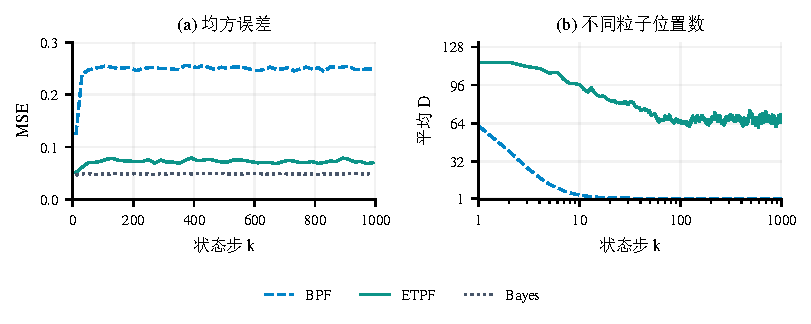
\includegraphics[width=0.88\linewidth]{figs/completed_work/logistic_robustness.pdf}
\caption{同一批运行的误差与粒子多样性。(a) 每 $20$ 步分段平均的 MSE 与 Bayes 参考风险；(b) 重采样后不同位置数的跨运行平均，横轴取对数以显示早期贫化。}
\label{cw:fig:sim-logistic-robustness}
\end{figure}
% 学位论文版式中正常续排结论，避免旧的预留空间指令将短段落推到新页。
BPF 的 $2048$ 次运行均贫化为单点；ETPF 在这批运行中没有单点贫化，末步平均保留 $69.67$ 个不同位置，总 MSE 较 BPF 降低 $70.9\%$。
这说明 ETPF 在本例中对无过程噪声下的粒子贫化更稳健。
